%%%%%%%%%%%%%%%%%%%%%%%%%%%%%%%%%%%%%%%%%%%%%%%%%%%%%%%%%%%%%%%%%
% Contents: Customising LaTeX output
% $Id: custom.tex,v 1.2 2003/03/19 20:57:45 oetiker Exp $
%%%%%%%%%%%%%%%%%%%%%%%%%%%%%%%%%%%%%%%%%%%%%%%%%%%%%%%%%%%%%%%%%
% 中文~4.20~翻译:zpxing@bbs.ctex  email: zpxing at gmail dot com
%%%%%%%%%%%%%%%%%%%%%%%%%%%%%%%%%%%%%%%%%%%%%%%%%%%%%%%%%%%%%%%%%

%\chapter{Customising \LaTeX}
\chapter{定制 \LaTeX}
\begin{intro}
%Documents produced with the commands you have learned up to this
%point will look acceptable to a large audience. While they are not
%fancy-looking, they obey all the established rules of good
%typesetting, which will make them easy to read and pleasant to look at.
到目前为止,运用你所学过的命令可以制作出能被绝大多数读者接受的文档。
尽管这些文档看上去不够奇妙,但它们遵循了高质量排版的已有规则,
这些规则可以使得文档易读,同时看起来也非常舒适。

%However, there are situations where \LaTeX{} does not provide a
%command or environment that matches your needs, or the output
%produced by some existing command may not meet your requirements.
然而在一些情况下,\LaTeX{} 也许并没有提供适合你需要的命令或者环境,
或者现有的命令产生的输出和你想要的不同。

%In this chapter, I will try to give some hints on
%how to teach \LaTeX{} new tricks and how to make it produce output
%that looks different from what is provided by default.
本章中,我将尝试给出一些新的技巧,运用这些技巧可以教会 \LaTeX{} 玩
一些新的把戏,也可以使得 \LaTeX{} 产生与众不同的输出。
\end{intro}


%\section{New Commands, Environments and Packages}
\section{新建命令、环境和宏包}
%You may have noticed that all the commands I introduce in this
%book are typeset in a box, and that they show up in the index at the end
%of the book. Instead of directly using the necessary \LaTeX{} commands
%to achieve this, I have created a \wi{package} in which I defined new
%commands and environments for this purpose. Now I can simply write:
你也许已经注意到我在这本书中介绍的所有命令都被包含在一个矩形框里,
并且出现在本书最后的索引中。 我并没有直接使用所需的 \LaTeX{} 命令
来实现这个,而是创建了一个宏包 (\wi{package}),并在其中定义了我
所需要的命令和环境。 现在我可以简单的写:

\begin{example}
\begin{lscommand}
\ci{dum}
\end{lscommand}
\end{example}

%In this example, I am using both a new environment called\\
%\ei{lscommand}, which is responsible for drawing the box around the
%command, and a new command named \ci{ci}, which typesets the command
%name and makes a corresponding entry in the index. You can check
%this out by looking up the \ci{dum} command in the index at the back
%of this book, where you'll find an entry for \ci{dum}, pointing to
%every page where I mentioned the \ci{dum} command.
在这个例子中,我使用了一个新的环境:\ei{lscommand}。这个环境负责在命令
的周围画出一个矩形框。同时我还使用了一个命令:\ci{ci}, 这个命令负责输出
命令的名字,并且在索引中添加相应的条目。你可以在本书最后的索引中查找命令 \ci{dum},
然后你会发现有一个 \ci{dum} 的条目,这个条目中列出了包含有 \ci{dum} 命令
的所有页的页码。

%If I ever decide that I do not like the commands to be typeset in
%a box any more, I can simply change the definition of the
%\texttt{lscommand} environment to create a new look. This is much
%easier than going through the whole document to hunt down all the
%places where I have used some generic \LaTeX{} commands to draw a
%box around some word.
一旦我不再喜欢在一个矩形框中排版命令,我可以轻松的
改变 \texttt{lscommand} 环境的定义,来创建新的外观。跟追踪并修改所有
使用原始的 \LaTeX{} 命令在文字周围画框的地方相比,这种做法容易得多。

%\subsection{New Commands}
\subsection{新建命令}

%To add your own commands, use the
%\begin{lscommand}
%\ci{newcommand}\verb|{|%
%       \emph{name}\verb|}[|\emph{num}\verb|]{|\emph{definition}\verb|}|
%\end{lscommand}
%\noindent command.
%Basically, the command requires two arguments: the \emph{name} of the
%command you want to create, and the \emph{definition} of the command.
%The \emph{num} argument in square brackets is optional and specifies the number
%of arguments the new command takes (up to 9 are possible).
%If missing it defaults to 0, i.e. no argument allowed.
为了建立你自己的命令,可以使用如下的命令:
\begin{lscommand}
\ci{newcommand}\verb|{|%
       \emph{name}\verb|}[|\emph{num}\verb|]{|\emph{definition}\verb|}|
\end{lscommand}
基本上,这个命令有两个参量,第一个 \emph{name} 是你想要建立的命令
的名称,第二个 \emph{definition} 是命令的定义。方括号里的参数 \emph{num} 是可选的,
用于指定新命令所需的参量数目(最多 9 个)。如果不给
出这个参数,默认就是 0,也就是新建的命令不要任何参量。

%The following two examples should help you to get the idea.
%The first example defines a new command called \ci{tnss}. This is
%short for ``The Not So Short Introduction to \LaTeXe.'' Such a command
%could come in handy if you had to write the title of this book over
%and over again.
接下来的两个例子有助你的理解。第一个例子定义了一个新的命令:\ci{tnss}。
这个命令是句子 ``The\ Not\ So\ Short\ Introduction\ to\ \LaTeXe'' 的简写。
如果你需要在文档中多次使用本书的名称,那么定义这个命令将是非常方便的。

\begin{example}
\newcommand{\tnss}{The not
    so Short Introduction to
    \LaTeXe}
This is ``\tnss'' \ldots{}
``\tnss''
\end{example}

%The next example illustrates how to define a new
%command that takes one argument.
%The \verb|#1| tag gets replaced by the argument you specify.
%If you wanted to use more than one argument, use \verb|#2| and
%so on.
下一个例子演示了如何建立一个接受单一参数的命令。在命令的定义中,标记 \verb|#1| 
将被你指定的参量所代替。如果你想使用多个参量,那么可以依次使用 \verb|#2|、……、
\verb|#9| 等标记。

\begin{example}
\newcommand{\txsit}[1]
 {This is the \emph{#1} Short
      Introduction to \LaTeXe}
% in the document body:
\begin{itemize}
\item \txsit{not so}
\item \txsit{very}
\end{itemize}
\end{example}

%\LaTeX{} will not allow you to create a new command that would
%overwrite an existing one. But there is a special command in case you
%explicitly want this: \ci{renewcommand}.
%It uses the same syntax as the \verb|\newcommand|
%command.
\LaTeX{} 不允许你新建一个与现有命令重名的命令。 如果你确实需要这么做,有一个专门
的命令用于处理这种情况:\ci{renewcommand}。它使用与命令 \verb|\newcommand| 
相同的语法。

%In certain cases you might also want to use the \ci{providecommand}
%command. It works like \ci{newcommand}, but if the command is
%already defined, \LaTeXe{} will silently ignore it.
在某些情况之下,你可能会希望使用 \ci{providecommand} 命令。它完成与 \ci{newcommand} 
命令相同的工作。但如果命令已经存在,\LaTeXe{} 将会悄悄忽略原有的那个。

%There are some points to note about whitespace following \LaTeX{} commands. See
%page \pageref{whitespace} for more information.
处理 \LaTeX{} 命令后尾随的空格有一些要注意的事项,参看第 \pageref{whitespace} 页
可以获得更多这方面的信息。

%\subsection{New Environments}
\subsection{新建环境}

%Just as with the \verb|\newcommand| command, there is a command
%to create your own environments. The \ci{newenvironment} command uses the
%following syntax:
与 \verb|\newcommand| 命令类似,有一个命令用于建立新的环境。这个命令就是
 \ci{newenvironment},它的语法如下所示:

\begin{lscommand}
\ci{newenvironment}\verb|{|%
       \emph{name}\verb|}[|\emph{num}\verb|]{|%
       \emph{before}\verb|}{|\emph{after}\verb|}|
\end{lscommand}

%Again \ci{newenvironment} can have
%an optional argument. The material specified
%in the \emph{before} argument is processed before the text in the
%environment gets processed. The material in the \emph{after} argument gets
%processed when the \verb|\end{|\emph{name}\verb|}| command is encountered.
同样地,\ci{newenvironment} 命有一个可选的
参量。在 \emph{before} 中的内容将在此环境包含的文本之前处理,而在
 \emph{after} 中的内容将在遇到 \verb|\end{|\emph{name}\verb|}| 命令时处理。

%The example below illustrates the usage of the \ci{newenvironment}
%command.
%\begin{example}
%\newenvironment{king}
% {\rule{1ex}{1ex}%
%      \hspace{\stretch{1}}}
% {\hspace{\stretch{1}}%
%      \rule{1ex}{1ex}}
%
%\begin{king}
%My humble subjects \ldots
%\end{king}
%\end{example}

下面的例子演示了 \ci{newenvironment} 命令的用法:
\begin{example}
\newenvironment{king}
{\rule{1ex}{1ex}%
     \hspace{\stretch{1}}}
{\hspace{\stretch{1}}%
     \rule{1ex}{1ex}}

\begin{king}
My humble subjects \ldots
\end{king}
\end{example}

%The \emph{num} argument is used the same way as in the
%\verb|\newcommand| command. \LaTeX{} makes sure that you do not define
%an environment that already exists. If you ever want to change an
%existing command, you can use the \ci{renewenvironment} command. It
%uses the same syntax as the \ci{newenvironment} command.
参量 \emph{num} 的使用方式与 \verb|\newcommand| 命令相同。\LaTeX{} 还同样保证你
不会不小心新建重名的环境。如果你确实希望改变一个现有的环境,你可以使用命令
 \ci{renewenvironment},它使用和命令 \ci{newenvironment} 相同的语法。

%The commands used in this example will be explained later. For the
%\ci{rule} command see page \pageref{sec:rule}, for \ci{stretch} go to
%page \pageref{cmd:stretch}, and more information on \ci{hspace} can be
%found on page \pageref{sec:hspace}.
在这个例子中用到一些命令将在随后解释:\ci{rule} 命令的解释可以参看第 \pageref{sec:rule} 页,
\ci{stretch} 命令的解释可以参看第 \pageref{cmd:stretch} 页,关于 \ci{hspace} 的
信息可以在第 \pageref{sec:hspace} 页找到。

%\subsection{Extra Space}
\subsection{额外的空白间距}

%When creating a new environment you may easily get bitten by extra spaces
%creaping in, which can potentially have fatal effects. For example when you
%want to create a title environemnt which supresses its own indentation as
%well as the one on the following paragraph. The \ci{ignorespaces} command in
%the begin block of the environment will make it ignore any space after
%executing the begin block. The end block is a bit more tricky as special
%processing occurs at the end of an environment. With the
%\ci{ignorespacesafterend} \LaTeX{} will issue an \ci{ignorespaces} after the
%special `end' processing has occured.
当创建新的环境时,你或许会为遇到额外的空白间距而烦扰,这些间距可能产生严重的后果。比如当你
建立一个标题环境,既不要自身的缩进也不要紧接着的下一段缩进时,在 begin 中加入
命令 \ci{ignorespaces} 会使新环境忽略执行 begin 之后遇到的一切空白间距,而 end 
就需要耍个小花招,因为我们要等到环境结束后才开始处理。使用 \ci{ignorespacesafterend},\LaTeX{} 会
在 end 处理完毕后,产生一个 \ci{ignorespaces}。

\begin{example}
\newenvironment{simple}%
 {\noindent}%
 {\par\noindent}

\begin{simple}
See the space\\to the left.
\end{simple}
Same\\here.
\end{example}

\begin{example}
\newenvironment{correct}%
 {\noindent\ignorespaces}%
 {\par\noindent%
   \ignorespacesafterend}

\begin{correct}
No space\\to the left.
\end{correct}
Same\\here.
\end{example}

%\subsection{Commandline \LaTeX}
\subsection{命令行的 \LaTeX}
%If you work on a Unix like OS, you might be using Makefiles to build your
%\LaTeX{} projects. In that connection it might be interesting to produce
%different versions of the same document by calling \LaTeX{} with commandline
%parameters. If you add the following structure to your document:
如果使用类 Unix 的操作系统工作,你可能会在使用 Makefiles 建立你的 \LaTeX{} 项目。
那样的话,用命令行参数操控 \LaTeX{} 来创建同一份文档的不同版本可是十分有趣的。如果
把下列配置写入你的文档:
\begin{verbatim}
\usepackage{ifthen}
\ifthenelse{\equal{\blackandwhite}{true}}{
  % "black and white" mode; do something..
}{
  % "color" mode; do something different..
}
\end{verbatim}

%Now you can call \LaTeX{} like this:
现在,你可以像这样来操作 \LaTeX{}:
\begin{verbatim}
latex '\newcommand{\blackandwhite}{true}% Drawing a graph
% Author: Stefan Kottwitz
% https://www.packtpub.com/hardware-and-creative/latex-cookbook
\documentclass[border=10pt]{standalone}
\usepackage{tkz-graph}
\GraphInit[vstyle = Shade]
\tikzset{
  LabelStyle/.style = { rectangle, rounded corners, draw,
                        minimum width = 2em, fill = yellow!50,
                        text = red, font = \bfseries },
  VertexStyle/.append style = { inner sep=5pt,
                                font = \Large\bfseries},
  EdgeStyle/.append style = {->, bend left} }
\thispagestyle{empty}
\begin{document}
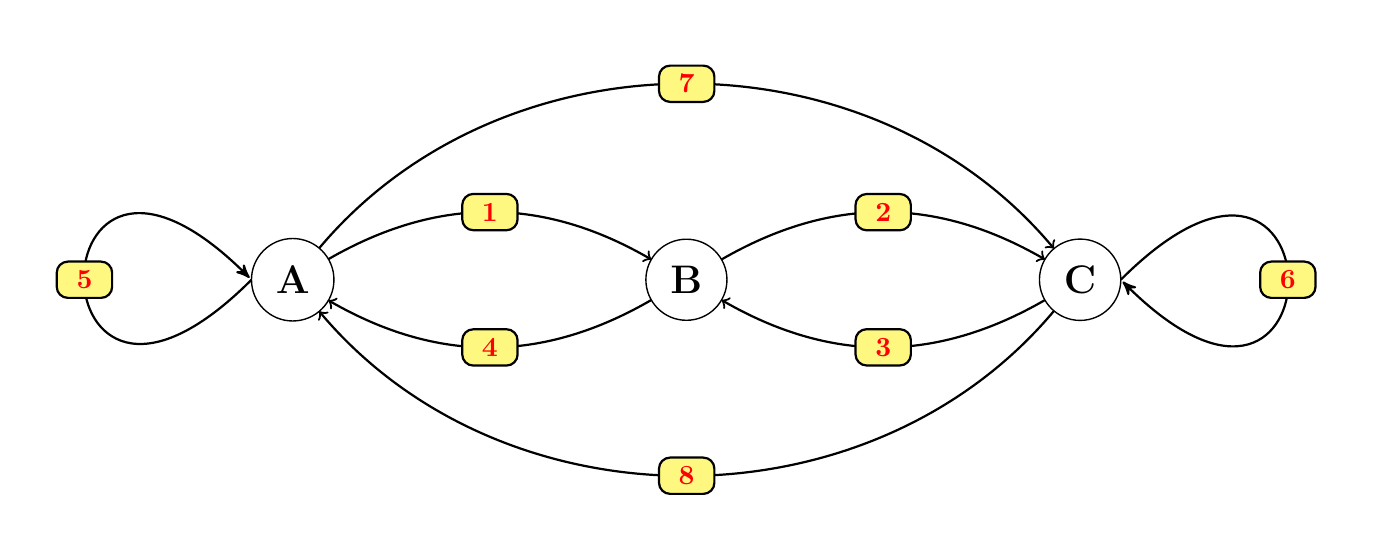
\begin{tikzpicture}
  \SetGraphUnit{5}
  \Vertex{B}
  \WE(B){A}
  \EA(B){C}
  \Edge[label = 1](A)(B)
  \Edge[label = 2](B)(C)
  \Edge[label = 3](C)(B)
  \Edge[label = 4](B)(A)
  \Loop[dist = 4cm, dir = NO, label = 5](A.west)
  \Loop[dist = 4cm, dir = SO, label = 6](C.east)
  \tikzset{EdgeStyle/.append style = {bend left = 50}}
  \Edge[label = 7](A)(C)
  \Edge[label = 8](C)(A)
\end{tikzpicture}
\end{document}'
\end{verbatim}

%First the command \verb|\blackandwhite| gets defined and then the actual file is read with input.
%By setting \verb|\blackandwhite| to false the color version of the document would be produced.
首先,定义命令 \verb|\blackandwhite|,然后使用 input 来读入实际的文档。要创建彩色版本文档,需要
设定 \verb|\blackandwhite| 为 false。

%\subsection{Your Own Package}
\subsection{自建宏包}

%If you define a lot of new environments and commands, the preamble of
%your document will get quite long. In this situation, it is a good
%idea to create a \LaTeX{} package containing all your command and
%environment definitions. You can then use the \ci{usepackage}
%command to make the package available in your document.
如果你定义了很多新的环境和命令,你的文档的导言部分将变得相当长,在这种情况下,
建立一个新的 \LaTeX{} 宏包来存放所有你自己定义的命令和环境将是一个好的处理方式。
然后你可以在文档中使用 \ci{usepackage} 命令来引入自定义宏包。

\begin{figure}[!htbp]
\begin{lined}{\textwidth}
\begin{verbatim}
% Demo Package by Tobias Oetiker
\ProvidesPackage{demopack}
\newcommand{\tnss}{The not so Short Introduction
                   to \LaTeXe}
\newcommand{\txsit}[1]{The \emph{#1} Short
                       Introduction to \LaTeXe}
\newenvironment{king}{\begin{quote}}{\end{quote}}
\end{verbatim}
\end{lined}
\caption{宏包样例。} \label{package}
\end{figure}

%Writing a package basically consists of copying the contents of
%your document preamble into a separate file with a name ending in
%\texttt{.sty}. There is one special command,
写一个宏包的基本工作就是将你原本很长的文档导言内容拷贝到另外一个的文件中去,
 这个文件需要以 \texttt{.sty} 结尾。你还加入一个专用的命令:
\begin{lscommand}
\ci{ProvidesPackage}\verb|{|\emph{package name}\verb|}|
\end{lscommand}
%\noindent for use at the very beginning of your package
%file. \verb|\ProvidesPackage| tells \LaTeX{} the name of the package
%and will allow it to issue a sensible error message when you try to
%include a package twice. Figure \ref{package} shows a small example
%package that contains the commands defined in the examples above.
\noindent 这个命令应该放在你的宏包的最前面。\verb|\ProvidesPackage| 告诉 \LaTeX{} 
宏包的名称从而让 \LaTeX{} 在你尝试两次引入同一个宏包的时候给出一个明显的
错误信息,图 \ref{package} 给出了一个小的宏包示例,其中包含了我们之前定义的一些命令。

%\section{Fonts and Sizes}
\section{字体和字号}

%\subsection{Font Changing Commands}
\subsection{字体变换命令}
%\index{font}\index{font size} \LaTeX{} chooses the appropriate font
%and font size based on the logical structure of the document
%(sections, footnotes, \ldots).  In some cases, one might like to change
%fonts and sizes by hand. To do this, you can use the commands listed in
%Tables \ref{fonts} and \ref{sizes}. The actual size of each font
%is a design issue and depends on the document class and its options.
%Table \ref{tab:pointsizes} shows the absolute point size for these
%commands as implemented in the standard document classes.
\index{font}\index{font size} \LaTeX{} 根据文档的逻辑结构(章节、脚注……)
来选择合适的字体和字体大小。在某些情况下,你可能会想要手动改变文档使用的
字体及其大小。为了完成这个目的,你可以使用表 \ref{fonts} 和表 \ref{sizes} 中
列出的那些命令。每个字体的实际大小是一个设计问题,并且它依赖于文档所使用
的文档类及其选项。表 \ref{tab:pointsizes} 列出了这些命令在标准文档类中的绝对 pt 大小。

\begin{example}
{\small The small and
\textbf{bold} Romans ruled}
{\Large all of great big
\textit{Italy}.}
\end{example}

%One important feature of \LaTeXe{} is that the font attributes are
%independent. This means that you can issue size or even font
%changing commands, and still keep the bold or slant attribute set
%earlier.
\LaTeXe{} 的一个重要特征是字体的各种属性是相互独立的,这意味着你可以改变字体
的大小而仍然保留字体原有的粗体或者斜体的特性。

%In \emph{math mode} you can use the font changing \emph{commands} to
%temporarily exit \emph{math mode} and enter some normal text. If you want to
%switch to another font for math typesetting you need another
%special set of commands; refer to Table \ref{mathfonts}.
在\textbf{数学模式}中你可以使用字体变换命令来暂时退出\textbf{数学模式},然后输入
一些正常的文字。如果你希望改变数学公式本身所使用的字体,\LaTeX{} 提供了另外一套命令。
参看表 \ref{mathfonts}。

\begin{table}[!bp]
\caption{字体。} \label{fonts}
\begin{lined}{12cm}
%
% Alan suggested not to tell about the other form of the command
% eg \verb|\sffamily| or \verb|\bfseries|. This seems a good thing to me.
%
\begin{tabular}{@{}rl@{\qquad}rl@{}}
\fni{textrm}\verb|{...}|        &      \textrm{\wi{roman}}&
\fni{textsf}\verb|{...}|        &      \textsf{\wi{sans serif}}\\
\fni{texttt}\verb|{...}|        &      \texttt{typewriter}\\[6pt]
\fni{textmd}\verb|{...}|        &      \textmd{medium}&
\fni{textbf}\verb|{...}|        &      \textbf{\wi{bold face}}\\[6pt]
\fni{textup}\verb|{...}|        &       \textup{\wi{upright}}&
\fni{textit}\verb|{...}|        &       \textit{\wi{italic}}\\
\fni{textsl}\verb|{...}|        &       \textsl{\wi{slanted}}&
\fni{textsc}\verb|{...}|        &       \textsc{\wi{Small Caps}}\\[6pt]
\ci{emph}\verb|{...}|          &            \emph{emphasized} &
\fni{textnormal}\verb|{...}|    &    \textnormal{document} font
\end{tabular}

\bigskip
\end{lined}
\end{table}


\begin{table}[!bp]
\index{font size} \caption{字号。} \label{sizes}
\begin{lined}{12cm}
\begin{tabular}{@{}ll}
\fni{tiny}      & \tiny        tiny font \\
\fni{scriptsize}   & \scriptsize  very small font\\
\fni{footnotesize} & \footnotesize  quite small font \\
\fni{small}        &  \small            small font \\
\fni{normalsize}   &  \normalsize  normal font \\
\fni{large}        &  \large       large font
\end{tabular}%
\qquad\begin{tabular}{ll@{}}
\fni{Large}        &  \Large       larger font \\[5pt]
\fni{LARGE}        &  \LARGE       very large font \\[5pt]
\fni{huge}         &  \huge        huge \\[5pt]
\fni{Huge}         &  \Huge        largest
\end{tabular}

\bigskip
\end{lined}
\end{table}

\begin{table}[!tbp]
\caption{标准文档类中的绝对 pt 大小。}\label{tab:pointsizes}
\label{tab:sizes}
\begin{lined}{12cm}
\begin{tabular}{lrrr}
\multicolumn{1}{c}{大小} &
\multicolumn{1}{c}{10pt (默认)} &
           \multicolumn{1}{c}{11pt 选项}  &
           \multicolumn{1}{c}{12pt 选项}\\
\verb|\tiny|       & 5pt  & 6pt & 6pt\\
\verb|\scriptsize| & 7pt  & 8pt & 8pt\\
\verb|\footnotesize| & 8pt & 9pt & 10pt \\
\verb|\small|        & 9pt & 10pt & 11pt \\
\verb|\normalsize| & 10pt & 11pt & 12pt \\
\verb|\large|      & 12pt & 12pt & 14pt \\
\verb|\Large|      & 14pt & 14pt & 17pt \\
\verb|\LARGE|      & 17pt & 17pt & 20pt\\
\verb|\huge|       & 20pt & 20pt & 25pt\\
\verb|\Huge|       & 25pt & 25pt & 25pt\\
\end{tabular}

\bigskip
\end{lined}
\end{table}


\begin{table}[!bp]
\caption{数学字体。} \label{mathfonts}
\begin{lined}{0.7\textwidth}
\begin{tabular}{@{}ll@{}}
\fni{mathrm}\verb|{...}|&     $\mathrm{Roman\ Font}$\\
\fni{mathbf}\verb|{...}|&     $\mathbf{Boldface\ Font}$\\
\fni{mathsf}\verb|{...}|&     $\mathsf{Sans\ Serif\ Font}$\\
\fni{mathtt}\verb|{...}|&     $\mathtt{Typewriter\ Font}$\\
\fni{mathit}\verb|{...}|&     $\mathit{Italic\ Font}$\\
\fni{mathcal}\verb|{...}|&    $\mathcal{CALLIGRAPHIC\ FONT}$\\
\fni{mathnormal}\verb|{...}|& $\mathnormal{Normal\ Font}$\\
\end{tabular}

%\begin{tabular}{@{}lll@{}}
%\textit{Command}&\textit{Example}&    \textit{Output}\\[6pt]
%\fni{mathcal}\verb|{...}|&    \verb|$\mathcal{B}=c$|&     $\mathcal{B}=c$\\
%\fni{mathscr}\verb|{...}|&    \verb|$\mathscr{B}=c$|&     $\mathscr{B}=c$\\
%\fni{mathrm}\verb|{...}|&     \verb|$\mathrm{K}_2$|&      $\mathrm{K}_2$\\
%\fni{mathbf}\verb|{...}|&     \verb|$\sum x=\mathbf{v}$|& $\sum x=\mathbf{v}$\\
%\fni{mathsf}\verb|{...}|&     \verb|$\mathsf{G\times R}$|&        $\mathsf{G\times R}$\\
%\fni{mathtt}\verb|{...}|&     \verb|$\mathtt{L}(b,c)$|&   $\mathtt{L}(b,c)$\\
%\fni{mathnormal}\verb|{...}|& \verb|$\mathnormal{R_{19}}\neq R_{19}$|&
%$\mathnormal{R_{19}}\neq R_{19}$\\
%\fni{mathit}\verb|{...}|&     \verb|$\mathit{ffi}\neq ffi$|& $\mathit{ffi}\neq ffi$
%\end{tabular}

\bigskip
\end{lined}
\end{table}

%In connection with the font size commands, \wi{curly braces} play a
%significant role. They are used to build \emph{groups}.  Groups
%limit the scope of most \LaTeX{} commands.\index{grouping}
使用字体命令的时候,大括号 (\wi{curly braces}) 扮演了一个重要角色。它们被用于
建立所谓的\textbf{组} (group)。组限制了大多数 \LaTeX{} 命令的作用范围。\index{grouping}

\begin{example}
He likes {\LARGE large and
{\small small} letters}.
\end{example}

%The font size commands also change the line spacing, but only if the
%paragraph ends within the scope of the font size command. The closing curly
%brace \verb|}| should therefore not come too early.  Note the position of
%the \ci{par} command in the next two examples. \footnote{\texttt{\bs{}par}
%is equivalent to a blank line}
如果段落在字体的作用范围中结束,那么字号命令还将改变段落中行距。因此
用于分组的反向大括号 \verb|}| 不应该太早出现。注意下面两个例子中
\ci{par} 命令的位置
\footnote{\texttt{\bs{}par} 相当于一个空行}。

\begin{example}
{\Large Don't read this!
 It is not true.
 You can believe me!\par}
\end{example}

\begin{example}
{\Large This is not true either.
But remember I am a liar.}\par
\end{example}

%If you want to activate a size changing command for a whole paragraph
%of text or even more, you might want to use the environment syntax for
%font changing commands.
如果你希望改变整段甚至更多文本的字体,你可能应该使用字体变换命令的环境语法。

\begin{example}
\begin{Large}
This is not true.
But then again, what is these
days \ldots
\end{Large}
\end{example}

%\noindent This will save you from counting lots of curly braces.
\noindent 这将使你从一堆大括号中解脱出来。

%\subsection{Danger, Will Robinson, Danger}
\subsection{战战兢兢,如履薄冰}

%As noted at the beginning of this chapter, it is dangerous to clutter
%your document with explicit commands like this, because they work in
%opposition to the basic idea of \LaTeX{}, which is to separate the
%logical and visual markup of your document.  This means that if you
%use the same font changing command in several places in order to
%typeset a special kind of information, you should use
%\verb|\newcommand| to define a ``logical wrapper command'' for the font
%changing command.
正如本章开头曾经说过的那样,在你的文档中直接运用这些命令来修改格式是非常
危险的事情,因为这种做法和 \LaTeX{} 的基础理念相反。在编写 \LaTeX{} 文档
的时候,要始终注意文章逻辑标记和样式标识的分离。也就是如果你在文
章的多个地方采用某种特殊的格式来排版一类经常使用的内容,
就应该使用 \verb|\newcommand| 来定义一个逻辑封装命令,并通过这个命令来修改相应的表现格式。

\begin{example}
\newcommand{\oops}[1]{%
 \textbf{#1}}
Do not \oops{enter} this room,
it's occupied by \oops{machines}
of unknown origin and purpose.
\end{example}

%This approach has the advantage that you can decide at some later
%stage that you want to use some visual representation of danger other
%than \verb|\textbf|, without having to wade through your document,
%identifying all the occurrences of \verb|\textbf| and then figuring out
%for each one whether it was used for pointing out danger or for some other
%reason.
这种方法具有一个明显的优点,你可以在以后决定使用一些不是很有把握实现的特别外观并
使之不同于 \verb|\textbf|,
那时你就不需要遍历你的整篇文章来找出所有 \verb|\textbf| 的地方,
然后一个一个地确定是不是要改成没有把握的外观。

%\subsection{Advice}
\subsection{建议}

%To conclude this journey into the land of fonts and font sizes,
%here is a little word of advice:\nopagebreak
总结这一章中关于字体和字号的命令,下面是一个简短的建议:\nopagebreak
%\begin{quote}
%  \underline{\textbf{Remember\Huge!}} \textit{The}
%  \textsf{M\textbf{\LARGE O} \texttt{R}\textsl{E}} fonts \Huge you
%  \tiny use \footnotesize \textbf{in} a \small \texttt{document},
%  \large \textit{the} \normalsize more \textsc{readable} and
%  \textsl{\textsf{beautiful} it bec\large o\Large m\LARGE e\huge s}.
%\end{quote}
\begin{quote}
 \underline{\textbf{Remember\Huge!}} \textit{The}
 \textsf{M\textbf{\LARGE O} \texttt{R}\textsl{E}} fonts \Huge you
 \tiny use \footnotesize \textbf{in} a \small \texttt{document},
 \large \textit{the} \normalsize more \textsc{readable} and
 \textsl{\textsf{beautiful} it bec\large o\Large m\LARGE e\huge s}.\\
 记住!你使用的字体越多,文章看起来就越易读越美观。
\end{quote}

%\section{Spacing}
\section{间距}

%\subsection{Line Spacing}
\subsection{行距}
%
%\index{line spacing} If you want to use larger inter-line spacing in a
%document, you can change its value by putting the
\index{line spacing}如果你想在文档中使用更大的行距,你可以在导言中使用
如下命令进行设定:
\begin{lscommand}
\ci{linespread}\verb|{|\emph{factor}\verb|}|
\end{lscommand}
%\noindent command into the preamble of your document.
%Use \verb|\linespread{1.3}| for ``one and a half'' line
%spacing, and \verb|\linespread{1.6}| for ``double'' line spacing.  Normally
%the lines are not spread, so the default line spread factor
%is 1.\index{double line spacing}
如 \verb|\linespread{1.3}| 产生 $1.5$ 倍行距,而 \verb|\linespread{1.6}| 
则产生双倍行距。缺省情况下的行距为 $1$。 \index{double line spacing}

%Note that the effect of the \ci{linespread} command is rather drastic and
%not appropriate for published work. So if you have a good reason for
%changing the line spacing you might want to use the command:
注意 \ci{linespread} 的效果相当夸张而且不适合出版工作。因此如果你很想改变行距
可能会希望使用如下的命令:
\begin{lscommand}
\verb|\setlength{\baselineskip}{1.5\baselineskip}|
\end{lscommand}

\begin{example}
{\setlength{\baselineskip}%
           {1.5\baselineskip}
This paragraph is typeset with
the baseline skip set to 1.5 of
what it was before. Note the par
command at the end of the
paragraph.\par}

This paragraph has a clear
purpose, it shows that after the
curly brace has been closed,
everything is back to normal.
\end{example}

%\subsection{Paragraph Formatting}\label{parsp}
\subsection{段落格式}\label{parsp}

%In \LaTeX{}, there are two parameters influencing paragraph layout.
%By placing a definition like
在 \LaTeX{} 中,有两个参数可以影响段落的布局。在文档的导言部分,可以通过
如下的定义来改变段落的布局。
\begin{code}
\ci{setlength}\verb|{|\ci{parindent}\verb|}{0pt}| \\
\verb|\setlength{|\ci{parskip}\verb|}{1ex plus 0.5ex minus 0.2ex}|
\end{code}
%in the preamble of the input file, you can change the layout of
%paragraphs. These two commands increase the space between two paragraphs
%while setting the paragraph indent to zero.
这两个命令增加了段落间距,并将首行缩进设置为 $0$。

%The \texttt{plus} and \texttt{minus} parts of the length above tell
%\TeX{} that it can compress and expand the inter paragraph skip by the
%amount specified, if this is necessary to properly fit the paragraphs
%onto the page.
例子中,长度设定中的 \texttt{plus} 和 \texttt{minus} 部分将使得 \TeX{} 按照指定大小
压缩和伸展段落间距。为了使得段落正确的显示在页面之上,\TeX{} 将在 0.8ex 
到 1.5ex 之间调整段落间距。

%In continental Europe,
%paragraphs are often separated by some space and not indented. But
%beware, this also has its effect on the table of contents. Its lines
%get spaced more loosely now as well. To avoid this, you might want to
%move the two commands from the preamble into your document to some
%place below the command \verb|\tableofcontents| or to not use them at all,
%because you'll find that most professional books use indenting and not
%spacing to separate paragraphs.
在欧洲大陆,段落通常用一些空白分隔并且一般首行不缩进。但是值得注意的是,这也会影响目录。
目录的行距也会变得非常疏松。为了避免这种情况,你可能需要将上面的两个命令从导言中移到文档
中 \verb|\tableofcontents| 以下适合的位置,或者根本不要使用这些,因为一般来说专业的书籍都是用缩进并且
通常不用空白来分离段落。
%
%If you want to indent a paragraph that is not indented, you can use
%\begin{lscommand}
%\ci{indent}
%\end{lscommand}
%\noindent at the beginning of the paragraph.\footnote{To indent the first paragraph after each section head, use
%  the \pai{indentfirst} package in the `tools' bundle.} Obviously,
%this will only have an effect when \verb|\parindent| is not set to
%zero.
如果你想缩进一个本来没有缩进的段落\footnote{为了缩进章节标题之后的第一个
段落,可以使用 \pai{indentfirst} 包。},可以在段落的开始使用命令:
\begin{lscommand}
\ci{indent}
\end{lscommand}
当然,这个命令只有在 \verb|\parindent| 不为零的情况下才有效果。

%To create a non-indented paragraph, you can use
%\begin{lscommand}
%\ci{noindent}
%\end{lscommand}
%\noindent as the first command of the paragraph. This might come in handy when
%you start a document with body text and not with a sectioning command.
为了创建一个不缩进的段落,你可以在段落的开始部分使用命令:
\begin{lscommand}
\ci{noindent}
\end{lscommand}
当文档以正文而不是章节命令开始的时候,这个命令会提供方便。

%\subsection{Horizontal Space}
\subsection{水平间距}
\label{sec:hspace}
\LaTeX{} 系统自动决定单词和句子之间的距离。为了增加水平距离,
使用命令:\index{horizontal!space}
\begin{lscommand}
\ci{hspace}\verb|{|\emph{length}\verb|}|
\end{lscommand}
%If such a space should be kept even if it falls at the end or the
%start of a line, use \verb|\hspace*| instead of \verb|\hspace|.  The
%\emph{length} in the simplest case is just a number plus a unit.  The
%most important units are listed in Table \ref{units}.
%\index{units}\index{dimensions}
如果这个水平间距即使在行首或者行末也应该保持的话,用命令 \verb|\hspace*| 代替 \verb|\hspace|。命令的 \emph{length} 参数在简单的情况下只是一个带有单位
的数字。最重要的长度单位在表 \ref{units} 中列了出来。
\index{units}\index{dimensions}

\begin{example}
This\hspace{1.5cm}is a space
of 1.5 cm.
\end{example}
\suppressfloats
\begin{table}[tbp]
\caption{\TeX{} 单位。} \label{units}\index{units}
\begin{lined}{9.5cm}
\begin{tabular}{@{}ll@{}}
\texttt{mm} & millimetre $\approx 1/25$ inch \quad \demowidth{1mm} \\
\texttt{cm} & centimetre = 10 mm  \quad \demowidth{1cm}                     \\
\texttt{in} & inch $=$ 25.4 mm \quad \demowidth{1in}                    \\
\texttt{pt} & point $\approx 1/72$ inch $\approx \frac{1}{3}$ mm  \quad\demowidth{1pt}\\
\texttt{em} & approx width of an `M' in the current font \quad \demowidth{1em}\\
\texttt{ex} & approx height of an `x' in the current font \quad \demowidth{1ex}
\end{tabular}

\bigskip
\end{lined}
\end{table}

%\label{cmd:stretch}
%The command
%\begin{lscommand}
%\ci{stretch}\verb|{|\emph{n}\verb|}|
%\end{lscommand}
%\noindent generates a special rubber space. It stretches until all the
%remaining space on a line is filled up. If two
%\verb|\hspace{\stretch{|\emph{n}\verb|}}| commands are issued on the
%same line, they grow according to the stretch factor.
\label{cmd:stretch}
下面的命令
\begin{lscommand}
\ci{stretch}\verb|{|\emph{n}\verb|}|
\end{lscommand}
\noindent 将产生一个特殊的橡皮长度:一个能把行内剩余所有空隙填满的空白。
如果两个 \verb|\hspace{\stretch{|\emph{n}\verb|}}| 命令位于同一行,那么它们将根据伸缩因子分配空间。

\begin{example}
x\hspace{\stretch{1}}
x\hspace{\stretch{3}}x
\end{example}

%When using horizontal space together with text, it may make sense to make
%the space adjust its size relative to the size of the current font.
%This can be done by using the text-relative units \texttt{em} and
%\texttt{ex}:
当在正文中使用水平间距的时候,相对于字号来调整间距大小会更有道理。这可以通过使用
与文本有关的单位 \texttt{em} 和 \texttt{ex} 来实现:
\begin{example}
{\Large{}big\hspace{1em}y}\\
{\tiny{}tin\hspace{1em}y}
\end{example}

%\subsection{Vertical Space}
\subsection{垂直间距}
%The space between paragraphs, sections, subsections, \ldots\ is
%determined automatically by \LaTeX. If necessary, additional vertical
%space \emph{between two paragraphs} can be added with the command:
在段落、节、小节…… 之间的距离是由 \LaTeX{} 系统自动决定的。如果必要的话,可以在两段之间
增加额外的距离,使用的命令如下所示:
\begin{lscommand}
\ci{vspace}\verb|{|\emph{length}\verb|}|
\end{lscommand}

%This command should normally be used between two empty lines.  If the
%space should be preserved at the top or at the bottom of a page, use
%the starred version of the command, \verb|\vspace*|, instead of \verb|\vspace|.
%\index{vertical space}
这个命令通常用于两个空行之间。如果这个额外的行距应该在于页的顶部和末尾也保留下来,那么使用
这个命令的星号版本 \verb|\vspace*| 来代替 \verb|\vspace|。
\index{vertical space}

%The \verb|\stretch| command, in connection with \verb|\pagebreak|, can
%be used to typeset text on the last line of a page, or to centre text
%vertically on a page.
命令 \verb|\stretch| 和 \verb|\pagebreak| 结合使用可以在页的最后一行输出文本,也可以
用来保证文本在页面上垂直居中。
\begin{code}
\begin{verbatim}
Some text \ldots

\vspace{\stretch{1}}
This goes onto the last line of the page.\pagebreak
\end{verbatim}
\end{code}

%Additional space between two lines of \emph{the same} paragraph or
%within a table is specified with the
\textbf{同一}段或\textbf{同一}个表格中两行之间的距离可以用如下命令来指定:
\begin{lscommand}
\ci{\bs}\verb|[|\emph{length}\verb|]|
\end{lscommand}
%\noindent command.

%With \ci{bigskip} and \ci{smallskip} you can skip a predefined amount of
%vertical space without having to worry about exact numbers.
使用命令 \ci{bigskip} 和 \ci{smallskip} 你可以获得一个预定义的垂直间距。

%\section{Page Layout}
\section{页面布局}

\begin{figure}[!hp]
\begin{center}
\makeatletter\@mylayout\makeatother
\end{center}
\vspace*{1.8cm}
\caption{页面布局参数。}
\label{fig:layout}
\cih{footskip}
\cih{headheight}
\cih{headsep}
\cih{marginparpush}
\cih{marginparsep}
\cih{marginparwidth}
\cih{oddsidemargin}
\cih{paperheight}
\cih{paperwidth}
\cih{textheight}
\cih{textwidth}
\cih{topmargin}
\end{figure}
%\index{page layout}
%\LaTeXe{} allows you to specify the \wi{paper size} in the
%\verb|\documentclass| command. It then automatically picks the right
%text \wi{margins}, but sometimes you may not be happy with
%the predefined values. Naturally, you can change them.
%%no idea why this is needed here ...
%\thispagestyle{fancyplain}
%Figure \ref{fig:layout} shows all the parameters that can be changed.
%The figure was produced with the \pai{layout} package from the tools bundle.%
%\footnote{\CTANref|macros/latex/required/tools|}
\index{page layout}
\LaTeXe{} 允许你在 \verb|\documentclass| 命令中指定纸张尺寸 (\wi{paper size})。
然后它将自动的选择合适的页边距。但有些时候你可能不满意 \LaTeX{} 的预设值,这个
时候你可以自己改变这些参数。
%no idea why this is needed here ...
\thispagestyle{fancyplain}
图 \ref{fig:layout} 中显示了所有能改变的页面参数。这个图是用 \pai{layout} 宏包
产生的\footnote{\CTANref|macros/latex/required/tools|}。

%\textbf{WAIT!} \ldots before you launch into a ``Let's make that
%narrow page a bit wider'' frenzy, take a few seconds to think. As with
%most things in \LaTeX, there is a good reason for the page layout to
%be as it is.
\textbf{先等等!} ……在你开始幻想“让这个狭窄的页面看起来宽一点”之前,先花一些时间
想想。和 \LaTeX{} 中的大多数规定一样,缺省的页面布局是有其合理原因的。

%Sure, compared to your off-the-shelf MS Word page, it looks awfully
%narrow. But take a look at your favourite book\footnote{I mean a real
%  printed book produced by a reputable publisher.} and count the number
%of characters on a standard text line. You will find that there are no
%more than about 66 characters on each line. Now do the same on your
%\LaTeX{} page. You will find that there are also about 66 characters
%per line.  Experience shows that the reading gets difficult as soon as
%there are more characters on a single line. This is because it is
%difficult for the eyes to move from the end of one line to the start of the next one.
%This is also why newspapers are typeset in multiple columns.
确实,相对于你的 MS\ Word 页面来说,它看上去非常的狭窄。但是看看你喜欢的书籍
\footnote{我说的是卓有声誉的出版商正式出版的书籍。}并且统计每个标准文本行的字符数目。
你会发现每行的字符不超过 66 个。现在你的 \LaTeX{} 页面也正是如此。经验显示,如果在
一行中塞入更多的字符,阅读将变得困难。这是因为眼睛从行的开始移动到行的结束变得困难了。
这也是报纸为何要排版成多栏形式的原因。

%So if you increase the width of your body text, keep in mind that you
%are making life difficult for the readers of your paper. But enough
%of the cautioning, I promised to tell you how you do it \ldots
因此如果你决定增加版芯的宽度,头脑中要明白你正在使给你的读者制造困难。警告已经
说的够多了,接下来我将告诉你如何去做……

%\LaTeX{} provides two commands to change these parameters. They are
%usually used in the document preamble.
\LaTeX{} 提供了两个命令来改变这些参数。他们通常在文章的导言部分使用。

%The first command assigns a fixed value to any of the parameters:
第一个命令给某些参数一个固定的值:
\begin{lscommand}
\ci{setlength}\verb|{|\emph{parameter}\verb|}{|\emph{length}\verb|}|
\end{lscommand}


%The second command adds a length to any of the parameters:
第二个命令给某些参数增加一个长度:
\begin{lscommand}
\ci{addtolength}\verb|{|\emph{parameter}\verb|}{|\emph{length}\verb|}|
\end{lscommand}

%This second command is actually more useful than the \ci{setlength}
%command, because you can now work relative to the existing settings.
%To add one centimetre to the overall text width, I put the
%following commands into the document preamble:
第二个命令实际上比 \ci{setlength} 命令更为实用,因为你可以相对于现有的设置来获得
所需的结果。为了给文本的宽度增加 1 厘米,我将如下的命令放置到文档导言:
\begin{code}
\verb|\addtolength{\hoffset}{-0.5cm}|\\
\verb|\addtolength{\textwidth}{1cm}|
\end{code}

%In this context, you might want to look at the \pai{calc} package.
%It allows you to use arithmetic operations in the argument of \ci{setlength}
%and other places where you can enter numeric values into function
%arguments.
这时候,你可能会想要看看 \pai{calc} 包,它允许你在 \ci{setlength} 的参量
中进行算术运算。它也可以运用到任何用数值作为函数参量的地方。


%\section{More Fun With Lengths}
\section{更有趣的长度}

%Whenever possible, I avoid using absolute lengths in
%\LaTeX{} documents. I rather try to base things on the width or height
%of other page elements. For the width of a figure this could
%be \verb|\textwidth| in order to make it fill the page.
只要可能,就应该避免在 \LaTeX{} 文档中使用绝对长度。我更愿意通过页面
中其他元素的宽度或高度来指定长度。比如一个图形,我指定 \verb|\textwidth| 作为
它的宽度从而使得图形恰好充满整个页面。

%The following 3 commands allow you to determine the width, height and
%depth of a text string.
下面的三个命令允许你获得一个文本串的宽度、高度以及深度。

\begin{lscommand}
\ci{settoheight}\verb|{|\emph{variable}\verb|}{|\emph{text}\verb|}|\\
\ci{settodepth}\verb|{|\emph{variable}\verb|}{|\emph{text}\verb|}|\\
\ci{settowidth}\verb|{|\emph{variable}\verb|}{|\emph{text}\verb|}|
\end{lscommand}

%\noindent The example below shows a possible application of these commands.
\noindent 下面的例子显示了如何应用这些命令:
\begin{example}
\flushleft
\newenvironment{vardesc}[1]{%
  \settowidth{\parindent}{#1:\ }
  \makebox[0pt][r]{#1:\ }}{}

\begin{displaymath}
a^2+b^2=c^2
\end{displaymath}

\begin{vardesc}{Where}$a$,
$b$ -- are adjoin to the right
angle of a right-angled triangle.

$c$ -- is the hypotenuse of
the triangle and feels lonely.

$d$ -- finally does not show up
here at all. Isn't that puzzling?
\end{vardesc}
\end{example}


%\section{Boxes}
\section{盒子}
%\LaTeX{} builds up its pages by pushing around boxes. At first, each
%letter is a little box, which is then glued to other letters to form
%words. These are again glued to other words, but with special glue,
%which is elastic so that a series of words can be squeezed or
%stretched as to exactly fill a line on the page.
\LaTeX{} 使用盒子来建立页面。首先,每个字符都是一个小的盒子,
这些盒子粘结起来构成单词,单词粘结起来构成一行。值得注意的是,单词
之间粘结的是一种特殊的“胶水” (glue),它是有弹性的,可以使 \LaTeX{} 压缩或者延伸使得单词将恰好构成页面的一行。

%I admit, this is a very simplistic version of what really happens, but
%the point is that \TeX{} operates on glue and boxes. Letters are not the only things that
%can be boxes. You can put virtually everything into a box, including
%other boxes. Each box will then be handled by \LaTeX{} as if it were a
%single letter.
我承认,这里的描述是实际情况一个极度简化了的版本,但关键在于 \TeX{} 
对盒子和胶水进行操作。不是只有字母才能成为盒子,你几乎可以把
任何东西包括其他盒子放到一个盒子中。 然后 \LaTeX{} 将会像处理
单个字母一样处理这个盒子。

%In the past chapters you have already encountered some boxes, although
%I did not tell you. The \ei{tabular} environment and the
%\ci{includegraphics}, for example, both produce a box. This means that you can
%easily arrange two tables or images side by side. You just have to
%make sure that their combined width is not larger than the textwidth.
在过去的章节中,尽管我并没有明确的说出来,你已经遇到了一些盒子。例如
 \ei{tabular} 环境和 \ci{includegraphics} 命令就都产生了一个盒子。这就
意味着你可以轻松的将两个表格或图像并列。你唯一需要保证的就是它们
宽度的总和不大于文本宽度。

%You can also pack a paragraph of your choice into a box with either
%the
使用如下命令可以把一个段落放置到盒子中:
\begin{lscommand}
\ci{parbox}\verb|[|\emph{pos}\verb|]{|\emph{width}\verb|}{|\emph{text}\verb|}|
\end{lscommand}

%\noindent command or the
\noindent 或者用下面这个环境完成同样的事情:

\begin{lscommand}
\verb|\begin{|\ei{minipage}\verb|}[|\emph{pos}\verb|]{|\emph{width}\verb|}| text
\verb|\end{|\ei{minipage}\verb|}|
\end{lscommand}

%\noindent environment. The \texttt{pos} parameter can take one of the letters
%\texttt{c, t} or \texttt{b} to control the vertical alignment of the box,
%relative to the baseline of the surrounding text. \texttt{width} takes
%a length argument specifying the width of the box. The main difference
%between a \ei{minipage} and a \ci{parbox} is that you cannot use all commands
%and environments inside a \ei{parbox}, while almost anything is possible in
%a \ei{minipage}.
参数 \texttt{pos} 可以取以下字符中的一个 \texttt{c}、\texttt{t}
 或 \texttt{b},
这个参数用于控制盒子相对周围文本基线的垂直方向对齐。\texttt{width} 是一个长度参量用于
调整盒子的宽度。\ei{minipage} 和 \ci{parbox} 的区别在于你可能无法在一个 \ei{parbox} 中使用所有的命令或者环境,而几乎任何东西都可以在 \ei{minipage} 中使用。

%While \ci{parbox} packs up a whole paragraph doing line breaking and
%everything, there is also a class of boxing commands that operates
%only on horizontally aligned material. We already know one of them;
%it's called \ci{mbox}. It simply packs up a series of boxes into
%another one, and can be used to prevent \LaTeX{} from breaking two
%words. As you can put boxes inside boxes, these horizontal box packers
%give you ultimate flexibility.
虽然\ci{parbox} 可以打包整个段落,完成分行在内的几乎所有事情,
\LaTeX{} 中还存在与此不同的另外一类盒子命令用于处理水平对齐的东西。我们已经知道其中的
一个 \pozhehao \ci{mbox},它只是简单地将其它盒子包含在一个盒子里,从而防止
 \LaTeX{} 断开两个单词。因为盒子中可以包含盒子,它可以给予作者几乎无限的灵活性。

\begin{lscommand}
\ci{makebox}\verb|[|\emph{width}\verb|][|\emph{pos}\verb|]{|\emph{text}\verb|}|
\end{lscommand}

%\noindent \texttt{width} defines the width of the resulting box as
%seen from the outside.\footnote{This means it can be smaller than the
%material inside the box. You can even set the
%width to 0pt so that the text inside the box will be typeset without
%influencing the surrounding boxes.}  Besides the length
%expressions, you can also use \ci{width}, \ci{height}, \ci{depth}, and
%\ci{totalheight} in the width parameter. They are set from values
%obtained by measuring the typeset \emph{text}. The \emph{pos} parameter takes
%a one letter value: \textbf{c}enter, flush\textbf{l}eft,
%flush\textbf{r}ight, or \textbf{s}pread the text to fill the box.
\noindent \texttt{width} 定义了生成的盒子的外部宽度\footnote{这意味着在盒子
内部看来,盒子的宽度可能会小一些,你甚至可以将盒子的宽度设置为 0\,pt,这样可以
使得盒子中的内容不影响其外部的布局。}。 除了长度表达式,你也可以传递
 \ci{width}、 \ci{height}、 \ci{depth} 和 \ci{totalheight} 给 \texttt{width}。
这几个值是测量盒子内部文本来获得的。参数 \emph{pos} 接受一个字符值:
\textbf{c} -- 居中、\textbf{l} -- 靠左、\textbf{r} -- 靠右和 \textbf{s} -- 
将文本均匀分布到整个盒子中。

%The command \ci{framebox} works exactly the same as \ci{makebox}, but
%it draws a box around the text.
命令 \ci{framebox} 和 \ci{makebox} 完成同样的工作,不同之处在于它在内部文本
的周围画出一个矩形框。

%The following example shows you some things you could do with
%the \ci{makebox} and \ci{framebox} commands.
下面的例子演示了你使用命令 \ci{makebox} 和 \ci{framebox} 能完成的一些工作:

\begin{example}
\makebox[\textwidth]{%
    c e n t r a l}\par
\makebox[\textwidth][s]{%
    s p r e a d}\par
\framebox[1.1\width]{Guess I'm
    framed now!} \par
\framebox[0.8\width][r]{Bummer,
    I am too wide} \par
\framebox[1cm][l]{never
    mind, so am I}
Can you read this?
\end{example}

%Now that we control the horizontal, the obvious next step is to go for
%  the vertical.\footnote{Total control is only to be obtained by
%  controlling both the horizontal and the vertical \ldots}
% No problem for \LaTeX{}. The
现在我们已经知道怎么控制盒子的水平方向长度了,接下来的步骤是学习如何控制
垂直方向\footnote{全面控制仅仅是水平方向控制和垂直方向控制的同时运用……}。
对于 \LaTeX{} 来说,轻而易举。命令

\begin{lscommand}
\ci{raisebox}\verb|{|\emph{lift}\verb|}[|\emph{extend-above-baseline}\verb|][|\emph{extend-below-baseline}\verb|]{|\emph{text}\verb|}|
\end{lscommand}

%\noindent command lets you define the vertical properties of a
%box. You can use \ci{width}, \ci{height}, \ci{depth}, and
%  \ci{totalheight} in the first three parameters, in order to act
%  upon the size of the box inside the \emph{text} argument.
\noindent 让你能够定义一个盒子在垂直方向的属性。在前面的三个参数中,
你可以使用 \ci{width}、\ci{height}、\ci{depth} 
和 \ci{totalheight},这样可以使得盒子的参数能够与盒子内部的文本匹配。

\begin{example}
\raisebox{0pt}[0pt][0pt]{\Large%
\textbf{Aaaa\raisebox{-0.3ex}{a}%
\raisebox{-0.7ex}{aa}%
\raisebox{-1.2ex}{r}%
\raisebox{-2.2ex}{g}%
\raisebox{-4.5ex}{h}}}
he shouted but not even the next
one in line noticed that something
terrible had happened to him.
\end{example}


%\section{Rules and Struts}
\section{标尺和支撑}
\label{sec:rule}

%A few pages back you may have noticed the command
很多页之前你可能注意到这样的命令:
\begin{lscommand}
\ci{rule}\verb|[|\emph{lift}\verb|]{|\emph{width}\verb|}{|\emph{height}\verb|}|
\end{lscommand}

%\noindent In normal use it produces a simple black box.
\noindent 通常它被用来输出一个简单的黑色盒子。

\begin{example}
\rule{3mm}{.1pt}%
\rule[-1mm]{5mm}{1cm}%
\rule{3mm}{.1pt}%
\rule[1mm]{1cm}{5mm}%
\rule{3mm}{.1pt}
\end{example}

%\noindent This is useful for drawing vertical and horizontal
%lines. The line on the title page, for example, has been created with a
%\ci{rule} command.
\noindent 这个命令可以用来产生水平方向和垂直方向的线条。例如标题页上的直线就是用一个 \ci{rule} 命令创建的。

%A special case is a rule with no width but a certain height. In
%professional typesetting, this is called a \wi{strut}. It is used to
%guarantee that an element on a page has a certain minimal height. You
%could use it in a \texttt{tabular} environment to make sure a row has
%a certain minimum height.
一种特殊的例子是没有宽度只有高度的标尺。在专业的出版中,这被称为支撑 (\wi{Struts})。
它被用来保证页面的某个元素具有一个确定的高度最小值。你可以在 \texttt{tabular} 环境中使用支撑
来使得某行具有一个特定的高度最小值。

\begin{example}
\begin{tabular}{|c|}
\hline
\rule{1pt}{4ex}Pitprop \ldots\\
\hline
\rule{0pt}{4ex}Strut\\
\hline
\end{tabular}
\end{example}

\bigskip
%{\flushright The End.\par}
{\flushright 全篇结束。\par}
%

% Local Variables:
% TeX-master: "lshort2e"
% mode: latex
% mode: flyspell
% End:
